The Server Side Application is the system responsible for producing a solution to a user request,
which corresponds to the specification of a resource, as described in section \ref{sec:api_protocol}.
Producing a solution to the user request involves the communcation with third party API's,
to obtain the necessary flight data, which is handled by the Data Management System,
detailed in section \ref{sec:dms_implementation}.
The actual production of a solution is managed by the Optimization System,
described in more detail in section \ref{sec:os_implementation}.
The architecture and implementation details of the SSA are 
presented in section \ref{sec:api_architecture},
and illustrated in figure \ref{fig:solution_steps}.


% \begin{figure}[H]
%   \centering
%   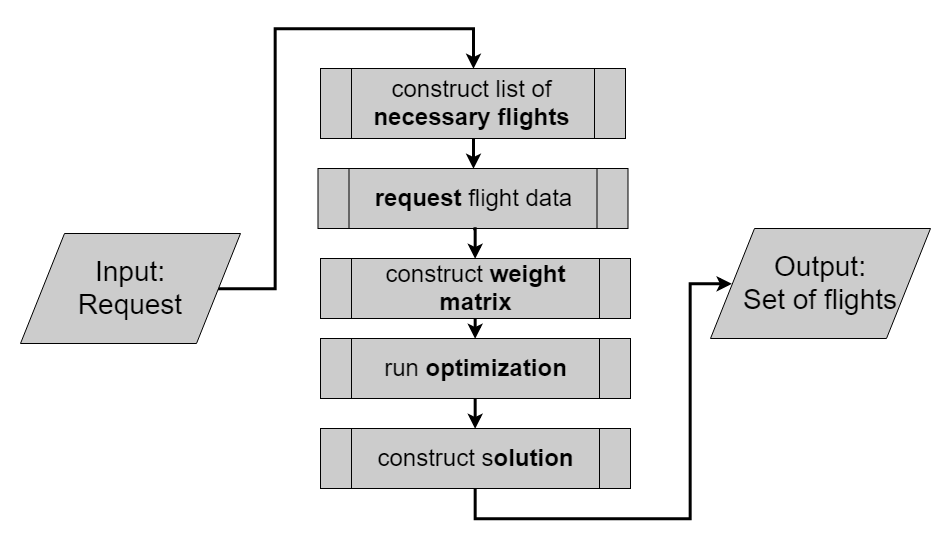
\includegraphics[width=\textwidth]{Figures/system_implementation/overall_flow_2.png}
%   \caption{Necessary steps to construct a solution to a user request.}
%   \label{fig:solution_steps}  
% \end{figure}